% Cahier des charges - Système de l'intervenant (PDA)
% Version 1.3

% Historique des versions
% 25/01/08 0.1 Version initiale
% 25/01/08 0.1.2 Plan remanié
% 27/01/08 0.2 Introduction/contexte et présentation des besoins
% 27/01/08 0.3 Exigences fonctionnelles
% 27/01/08 0.3.5 Grille d'analyse exigences fonctionnelles et planning
% 28/01/08 0.9 Quasiment tout, pas relu
% 29/01/08 1.0 Configuration cible, vite fait relu
% 29/01/08 1.1 Relecture OK par Nico
% 29/01/08 1.2 Modifications post-présentation
% 29/01/08 1.2.5 Ajout du découpage applicatif (schéma)
% 01/02/08 1.3 Document relu et validé

\documentclass[a4paper, 11pt, final]{article}

\usepackage[utf8]{inputenc} % Texte en utf-8
\usepackage{aeguill} % Coupure des mots accentués
\usepackage[francais]{babel} % Typographie française
\usepackage[pdftex, hypertexnames=false, colorlinks=true, final]{hyperref}
\usepackage[final]{graphicx}
\usepackage{url} % Gestion des URLs
\usepackage{geometry}
\usepackage{placeins} % Meilleur placement des images et tableaux
\usepackage{fancyhdr}
\usepackage[Lenny]{fncychap}

% Marges à gauche et à droite de 3cm
\geometry{margin=3cm}

% Utilisation des headers et footers personnalisés de fancyhdr
\pagestyle{fancy}

% Images dans le dossier ./images/
\graphicspath{{./images/}}

% Gestion des métadonnées étranges à rendre visibles au rendu
\newcommand\docname{CDCSIv1.3}
\newcommand\docauthor{Nicolas Kandel}
\newcommand\docstatus{LIVRABLE} % EN COURS, ATTENTE, VALIDE ou LIVRABLE

% Numérotation mieux
%\renewcommand\thechapter{\Alph{chapter}}
%\renewcommand\thesection{\Roman{section}}
%\renewcommand\thesubsection{\arabic{subsection}}
%\renewcommand\thesubsubsection{\alph{subsubsection}}

% Format de citation de références standard, marche avec quasiment tout
\newcommand\fullref[1]{\ref{#1}, page \pageref{#1}}

% En-têtes et pieds de page
\lhead{\docname}
\rhead{}
\lfoot{Auteur : H4213}
\cfoot{}
\rfoot{\thepage}

% Titre du document maître
\title{\textbf{COPEVUE}\\
\rule{\textwidth}{1pt}{}\\
\Huge{\textsc{Cahier des charges\\Système de l'intervenant}}}
\author{\docauthor{} (H4213)}
\date{\docname{} --- \today{} (\docstatus{})}

\begin{document}

\maketitle

\tableofcontents

\pagebreak

\section{Introduction}

\subsection{Rappel du contexte}
Il existe aujourd'hui de nombreux sites isolés et/ou difficiles d'accès qui nécessitent une surveillance et parfois des actions à distance. Ces sites se situent dans des espaces très différents tels que les citernes placées dans les forêts escarpées du pourtour méditerranéen, les réservoirs utilisés pour l'autonomie des chantiers dans le grand Nord mais aussi les personnes âgées qui se retrouvent souvent isolées.

Actuellement tous les contrôles et actions sont réalisés par un opérateur qui doit se déplacer sur le site. Il n'y a donc que très peu de réactivité, on ne peut pas avoir un suivi fin des évolutions et des problèmes graves~-- par exemple la fuite d'un réservoir~-- ne peuvent pas être traités rapidement.

\paragraph{Étude COPEVUE}
L'objet de l'étude est la mise en place d'un système générique de surveillance et d'action à distance sur des sites isolés. Le système devra être évolutif, autonome et fiable.

\subsection{Présentation du document}
Ce document présente le cahier des charges du système de l'intervenant. Cette sous-partie du système global permet à un intervenant en déplacement de recevoir et d'envoyer des informations aux sites isolés et/ou au système central. En pratique, ces actions se feront à l'aide d'un PDA ou d'un téléphone portable, système que l'on nommera génériquement \textit{smartphone}.

Dans le cadre du logiciel à développer, le cahier des charges sert de base à la rédaction des clauses contractuelles techniques de qualité et de réception, à partir desquelles le réalisateur proposera les spécifications fonctionnelles et non fonctionnelles du futur logiciel. Ce sont les besoins logiciels.

Nous exprimerons ces besoins en termes d'obligation de résultats, pas d'exigence de moyens. Ce document situe l'importance des fonctions du produit à développer pour l'application destinée au système de l'intervenant et donne leurs critères d'appréciation.

\subsection{Documents applicables et de référence}
\paragraph{Documents applicables}
\begin{itemize}
\item Dossier de gestion de la documentation
\item Dossier de spécification technique des besoins
\item Dossier de faisabilité
\end{itemize}

\paragraph{Documents de référence}
\begin{itemize}
\item Plan de référence d'un cahier des charges
\end{itemize}


\section{Présentation des besoins du logiciel}
% Expression des besoins à satisfaire, but, principe du logiciel
% besoins, exploitation et ergonomie, expérience
% portée, développement, mise en oeuvre, organisation de la maintenance
% limites

\subsection{Objectifs du logiciel}
Le logiciel que nous développons doit permettre à un intervenant en déplacement de recevoir et d'envoyer des informations/configurations aux sites isolés et/ou au système central, ceci à l'aide d'un \emph{smartphone}.

On peut relever trois catégories d'utilisation distinctes : les demandes liées à la géographie~-- localisation, consultation d'itinéraires~-- les commandes à effectuer sur les systèmes isolés et central~-- test de capteur, vérifications diverses~--  et un module de communication~-- envoi et réception de courriels.

\subsubsection{Géopositionnement}
La première catégorie d'utilisation est une aide pour l'intervenant, en particulier dans les cas de déplacement sur site pour une maintenance non technique ou informatique. Elle concerne \textit{a priori} l'intervenant devant gérer une panne de l'alimentation électrique ou s'occupant du réapprovisionnement en matières premières. Cependant, les intervenants techniciens auront eux aussi intérêt à utiliser ce service pour renseigner leur position et effectuer des demandes d'itinéraires, en particulier lors d'interventions urgentes nécessitant un technicien sur place.

\subsubsection{Intervention sur site}
Lors des interventions techniques, l'intervenant doit pouvoir se connecter sur le système local. Il doit pouvoir communiquer avec le matériel~-- capteurs et actionneurs~-- présent dans un but de maintenance préventive et en cas de panne. Il pourra ainsi effectuer une batterie de tests pour valider le bon fonctionnement du système. Il sera capable de se connecter au système central pour rendre compte de son intervention et vérifier que le pilotage du site isolé à distance est assuré.

\subsubsection{Communication}
Le système de l'intervenant est aussi un moyen de communication avec l'intervenant. Il est nécessaire de savoir à chaque instant la situation géographique de chaque intervenant et de pouvoir entrer en contact avec eux. Un système de communication textuel~-- type courriel~-- sera mis en place afin de prévenir l'intervenant d'un changement d'objectif, d'une intervention urgente et plus prioritaire, etc.

\subsection{Contraintes liées au contexte}

\subsubsection{Expérience utilisateur}
Nous avons vu qu'il existe deux types d'utilisateurs : les intervenants de maintenance non technique et les techniciens. Leur expérience en informatique étant différente, le logiciel développé doit tenir compte de cette contrainte et satisfaire tous les utilisateurs. Les techniciens ayant une expérience utilisateur correcte dans le domaine de l'informatique, nous pouvons nous permettre de privilégier les fonctionnalités à l'ergonomie pour le module d'\emph{Intervention sur site}. Ce n'est pas le cas pour les modules de \emph{Géopositionnement} et de \emph{Communication} qui seront aussi utilisés par des non techniciens moins habitués aux outils informatiques. Ces modules devront être facilement pris en main, d'autant plus qu'ils proposeront des services simples et prédéfinis.

\subsubsection{Ergonomie générale}
L'ergonomie générale doit tenir compte de deux contraintes majeures : la plateforme de destination est portable et une partie des utilisateurs n'a pas beaucoup d'expérience dans le maniement des outils informatiques.

Notre logiciel doit permettre un accès rapide et simple à chacun des modules dès l'identification de l'intervenant. Les services proposés seront eux aussi regroupés par catégorie afin de permettre une utilisation intuitive.

Les modules de \emph{Géopositionnement} et de \emph{Communication} proposeront un accès exhaustif à leurs fonctionnalités alors que la relative complexité de l'interface de gestion des \emph{Interventions sur site} proposera une interface moins intuitive mais plus puissante, d'autant plus que la liste des fonctionnalités ne peut être exhaustive.

\subsection{Découpage applicatif}

L'application à destination du système de l'intervenant est composée de trois modules fonctionnels.

\begin{figure}[!h]
\begin{center}
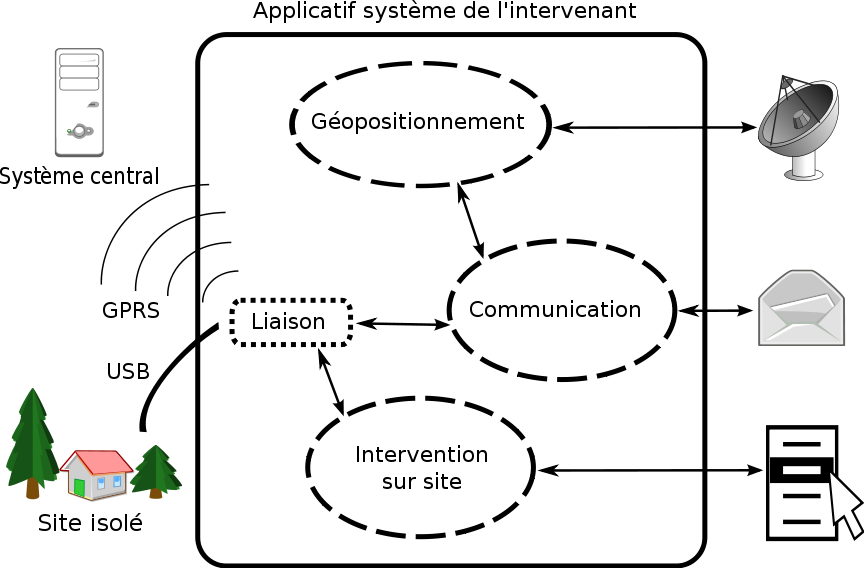
\includegraphics[width=\textwidth]{schema_modules_pda.png}
\caption{Découpage applicatif du système de l'intervenant}
\end{center}
\end{figure}

On note la présence du bloc applicatif \emph{Liaison} qui est une couche d'abstraction gérant les différentes communications~-- au sens réseau et non partage d'informations~-- avec les systèmes extérieurs à celui de l'intervenant : \emph{système central} et \emph{sites isolés}.

\section{Exigences fonctionnelles}
% fonctions, performances, facteurs de qualité

\subsection{Envoi position intervenant}
Envoie au système central la position de l'intervenant. Cet envoi est invisible à l'utilisateur, il se fait en réponse à la demande de position effectuée par le serveur central. L'envoi est à la charge du système de l'intervenant, la position est récupérée par une balise GPS ou par le \emph{smartphone} lui-même. La demande de position et son envoi se font par courriel non notifié à l'utilisateur.

\subsection{Demande itinéraire}
Envoie une requête de demande d'itinéraire au système central. Cet itinéraire est calculé par ce dernier en fonction de la position de l'intervenant et du lieu de destination.

\subsection{Affichage itinéraire}
Affiche à l'écran du système de l'intervenant un itinéraire. À la vue des limitations du débit proposé par le réseau GPRS, l'itinéraire sera un fichier texte structuré en XML. Il transitera \textit{via} le réseau GPRS par courriel compressé. Il appartient au logiciel approprié de présenter un itinéraire graphique. L'affichage et les informations contextuelles dépendra de la plateforme utilisée par l'intervenant.

\subsection{Identification}
Réalise une identification centralisée pour accéder au serveur central ainsi qu'aux sites isolés. Celle-ci requiert une authentification qui se fera à l'aide du système clef publique/clef privée RSA.

\subsection{Connexion distante au site isolé}
Effectue une connexion distante au site isolé afin d'accéder à l'ensemble des fonctions que propose le système embarqué. De cette manière, l'intervenant pourra ajouter/supprimer/configurer des capteurs/actionneurs, procéder à des tests de lecture et d'activation, configurer et redémarrer le système embarqué. Cette connexion distante est sécurisée et passe par le système central~-- cas de fonctionnement standard.

\subsection{Connexion locale au site isolé}
Effectue une connexion locale au site isolé afin d'accéder à l'ensemble des fonctions que propose le système embarqué. Ce type de connexion permet le même accès qu'une connexion distante, il est utilisé en cas de panne et/ou de défaillance de la connexion distante et sert principalement à diagnostiquer, configurer et redémarrer le système embarqué.

% \subsection{Ajout capteur/actionneur}
%
% \subsection{Suppression capteur/actionneur}
%
% \subsection{Redémarage capteur/actionneur}
%
% \subsection{Lecture valeur capteur}
%
% \subsection{Activation actionneur}
%
% \subsection{Configuration capteur/actionneur}
%
% \subsection{Configuration système embarqué}
%
% \subsection{Redémarage système embarqué}

\subsection{Envoi rapport d'intervention}
Permet l'envoi d'un rapport d'intervention, notamment en cas de connexion locale au site isolé où aucun évènement n'a pu être enregistré par le serveur du système central.

\subsection{Envoi message}
Envoi de message textuel type courriel au système central, le contenu du message ainsi que le destinataire final ne sont pas sous contraintes.

\subsection{Réception message}
Gère une boîte de réception de messages textuels type courriel propre au système de l'intervenant et à son propriétaire.

% \subsection{Connexion internet}

% \subsection{Alarme}


\section{Exigences non fonctionnelles}
% sûreté, faisabilité, planning, organisation, interfaces
% == contraintes non fonctionnelles

\subsection{Sécurité}
Bien que les risques d'espionnage des communications entre sites et système de l'intervenant sont relativement restreints, nous devons assurer une certaine robustesse afin d'éviter les attaques les plus courantes. Dans ce sens, nous appliquerons une politique de sécurité stricte qui prend en compte une identification centralisée, une authentification et l'utilisation de protocoles de communication cryptés fiables.

\subsection{Fiabilité}
La fiabilité des applications installées sur le système de l'intervenant doit être exemplaire. Nous ne pouvons pas nous permettre de bloquer le \textit{smartphone} de l'intervenant au cous d'une opération importante. Le logiciel développé devra faire preuve d'un haut niveau de fiabilité et de résistance aux erreurs.

\subsection{Ergonomie}
L'ergonomie du logiciel développé devra être adaptée aux deux groupes d'utilisateurs définis dans les \textit{contraintes liées au contexte} : les intervenants techniciens et non techniciens. Les modules \emph{Géopositionnement} et \emph{Communication} doivent être simples, exhaustifs et rapides ; le module d'\emph{Intervention sur site} doit être axé sur les fonctionnalités. Les différentes interfaces suivront les principes d'ergonomie épurée. L'utilisation d'onglets est recommandée pour les plateformes de type \textit{smartphones}.

\subsection{Portabilité}
Dès la phase de conception de l'application, il faudra prendre en compte la multiplicité des plate-formes de destination. Une application pour \textit{smartphones} doit être ultraportable et évolutive car nous ne savons pas à l'avance sur quels modèles de PDA ou de téléphones mobiles elle sera installée à l'avenir.

\subsection{Modularité}
Une modularité de développement~-- séparer distinctement les couches de transfert de données, d'acquisition, etc.~-- permettra de s'adapter aux différents systèmes de l'intervenant. On pourra utiliser par exemple une acquisition au clavier pour les téléphones portables et l'utilisation d'un écran tactile pour les PDA.

\subsection{Configuration}
Le \textit{smartphone} étant l'outil de travail de l'intervenant, nous prévoyons de rendre l'application qu'il utilise au quotidien un minimum configurable. Les options de configuration attendues sont celles fréquemment rencontrées dans ce type de logiciel, leur présence dépendra de leur facilité d'implémentation.

\subsection{Performances et facteurs de qualité}
Le développement du logiciel devra enfin prendre en compte des exigences de performances tout en intégrant d'importants facteurs de qualité. Ceci concerne par exemple la gestion des pannes étudiée en amont des phases de conception, l'utilisation de protocoles éprouvés, etc. Le but est d'atteindre des performances correctes tout en garantissant une stabilité logicielle.


\section{Analyse des exigences}
% tableaux avec la liste des exigences confrontées à l'importance et à la faisabilité

\subsection{Critères d'analyse}
Chacune des exigences fonctionnelles et non fonctionnelles est analysée et évaluée selon deux critères : sa nécessité et sa difficulté d'implémentation. Il lui est attribué deux notes sur 10, 0 signifiant par exemple la faisablité la plus basse et 10 l'importance la plus haute.

\subsection{Analyse des exigences fonctionnelles}

\paragraph{}
\begin{figure}[h!]
\begin{center}
\begin{tabular}{|r|c|c|}
\hline
Fonction & Nécessité & Difficulté d'implémentation\\ \hline \hline
Envoi position intervenant & 8 & 5\\ \hline
Demande itinéraire & 7 & 8\\ \hline
Affichage itinéraire & 7 & 8\\ \hline
Identification & 8 & 6\\ \hline
Connexion distante au site isolé & 9 & 5\\ \hline
Connexion locale au site isolé & 9 & 4\\ \hline
Envoi rapport d'intervention & 5 & 3\\ \hline
Envoi message & 8 & 3\\ \hline
Réception message & 8 & 3\\ \hline
\end{tabular}
\end{center}
\caption{Grille d'analyse des exigences fonctionnelles}
\end{figure}
\FloatBarrier

% \pagebreak

\subsection{Analyse des exigences non fonctionnelles}

\paragraph{}
\begin{figure}[h!]
\begin{center}
\begin{tabular}{|r|c|c|}
\hline
Fonction & Nécessité & Difficulté d'implémentation\\ \hline \hline
Sécurité & 7 & 6\\ \hline
Fiabilité & 8 & 8\\ \hline
Ergonomie & 6 & 6\\ \hline
Portabilité & 8 & 7\\ \hline
Modularité & 8 & 8\\ \hline
Configuration & 3 & 6\\ \hline
Performances et facteurs de qualité & 7 & 7\\ \hline
\end{tabular}
\end{center}
\caption{Grille d'analyse des exigences non fonctionnelles}
\end{figure}
\FloatBarrier


\section{Mise en œuvre}

\subsection{Faisabilité}
À la vue des analyses des exigences fonctionnelles et non fonctionnelles, en prenant en compte l'existant logiciel satisfaisant ou se rapprochant de nos contraintes de contexte, la faisabilité du logiciel pilotant le système de l'intervenant est approuvée.

\subsection{Configuration cible}

\subsubsection{Matériel}
Le matériel requis n'est pas soumis à de fortes contraintes. Il peut s'agir d'un PDA tout comme d'un téléphone mobile, voire d'un ordinateur portable. Ce qui importe est que le \textit{smartphone} soit assez récent et puissant pour faire tourner le logiciel cible avec son environnement et qu'il propose les périphériques et la connectique nécessaire. Dans la pratique, le matériel cible recherché pourrait être un PDA doté d'un large écran couleur, disposant d'un clavier physique et datant de moins d'un an.

\subsubsection{Environnement opérationnel}
L'environnement de l'application à développer n'est pas un critère. Cette application doit être multi-plateforme dans un souci de portabilité entre les \textit{smartphones} se basant sur différentes plateformes~-- Windows mobile, Unix, Java, etc. Pour permettre cette portabilité, l'environnement opérationnel doit permettre l'exécution de programmes codés dans des langages de haut niveau~-- Java 1.5, Python 2.5, etc.

\subsubsection{Connectique}
Les \emph{smartphones} des intervenants nécessiteront :
\begin{description}
\item[une connectique USB] pour une liaison filaire avec les sites isolés,
\item[une connectique GSM/GPRS] pour accéder aux possibilités de téléphonie et accéder à distance aux informations du système central et des sites à distance,
\item[une connectique GPS] pour suivre la position des intervenants à distance, celle-ci est optionnelle si le \emph{smartphone} dispose d'un système de géolocalisation par réseau GSM.
\end{description}

\pagebreak

\subsection{Planning}
Le planning de développement de notre application est donné ci-après. Il est prévisionnel et ne prend pas en compte les phases de déploiement ni celles de formation des intervenants. Ce planning est donné à titre indicatif dans un souci d'intégration au système global, il n'est pas à prendre comme contrainte de développement~-- notamment dans le cas d'une réponse à une appel d'offre.

\begin{figure}[h!]
\begin{center}
\begin{tabular}{|p{9cm}|c|}
\hline
Phase & Durée prévisionnelle\\ \hline \hline
Développement et tests unitaires & 6 mois\\ \hline
Tests en simulation et tests d'intégration & 3 mois\\ \hline
Tests avec matériel et retour d'expérience & 2 mois\\ \hline
Finalisation, éventuellement reprise de code posant des erreurs ou modifications logicielles dans un souci d'améliorer l'ergonomie, le retour d'expérience nous indiquant les lacunes à combler & 3 mois\\ \hline
Total & 14 mois\\ \hline
\end{tabular}
\end{center}
\caption{Planning prévisionnel de livraison du logiciel à destination du système distant}
\end{figure}
\FloatBarrier

% \appendix

% \section{Étude préalable}
% étude de l'existant, contexte du logiciel dans la société du demandeur

% rien

% \section{Étude de faisabilité}
% élaboration des solutions possibles

% cf Étude de faisabilité}

\end{document}
